\section{Lines in $\R^3$}

We now put the polynomial method of \Cref{Ch7:Sec:Polynomial_Method} to work, starting with lines in $\R^3$.

\begin{boxdefinition}[Joint]
    A \textbf{joint} in $\R^3$ is an intersection point of $3$ non-coplanar lines.
\end{boxdefinition}

In other words, any point at which three lines that do not share a plane in common meet is called a joint.

We ask ourselves the following question: how many joints can a collection of $L$ lines have?

Let's denote the greatest such number $J(L)$.

Here's one construction: just an $n \times n \times n$ grid. This gives you $3n^2$ lines and $n^3$ joints.

\begin{figure}[H]
    \centering
    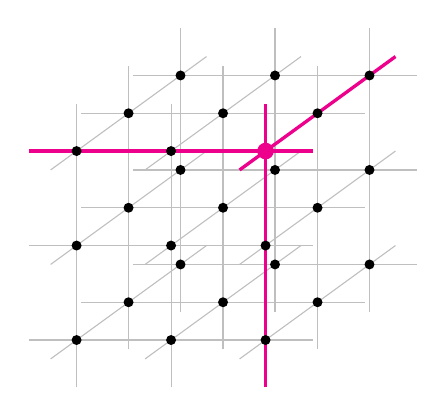
\begin{tikzpicture}[x = {(1cm, 0cm)}, y = {(0.55cm, 0.4cm)}, z = {(0cm, 1cm)}, scale = 1.2]
        \foreach \a in {0, 1, 2}{
            \foreach \b in {0, 1, 2}{
                \draw[gray!50] (-0.5, \a, \b) -- (2.5, \a, \b);
                \draw[gray!50] (\a, -0.5, \b) -- (\a, 2.5, \b);
                \draw[gray!50] (\a, \b, -0.5) -- (\a, \b, 2.5);
            }
        }
        \draw[very thick, magenta] (-0.5, 0, 2) -- (2.5, 0, 2);
        \draw[very thick, magenta] (2, -0.5, 2) -- (2, 2.5, 2);
        \draw[very thick, magenta] (2, 0, -0.5) -- (2, 0, 2.5);
        \foreach \a in {0, 1, 2}{
            \foreach \b in {0, 1, 2}{
                \foreach \c in {0, 1, 2}{
                    \fill[black] (\a, \b, \c) circle (1.5pt);
                }
            }
        }
        \fill[magenta] (2, 0, 2) circle (2.5pt);
    \end{tikzpicture}
\end{figure}
The case $n = 3$ is drawn above, with the three lines through one of the joints highlighted.

To bound $J(L)$ from above, we show that some line is always in few joints.

\begin{boxlemma}
    In any collection of $L$ lines, some line participates in $\leq 3J^{\frac{1}{3}}$ joints.
\end{boxlemma}
\begin{proof}
    Suppose not. Ie, suppose we have a collection of $L$ lines in which every line participates in $> 3 J^{\frac{1}{3}}$ joints.
    
    % [CORRECTED] was: "$D \leq J^{\frac{1}{3}}$" --- the lemma cited gives $3J^{\frac{1}{3}}$, which is the bound used below; $J^{\frac{1}{3}}$ fails for the six edges of a tetrahedron ($J = 4$, $D = 2$)
    Consider a nonzero polynomial $p$ over $\R$ in $3$ variables of the least degree $D \leq 3J^{\frac{1}{3}}$ that vanishes on the joints. Such a polynomial exists by \Cref{Ch7:Lemma:Low_Degree_Vanishing}.

    We've assumed every line in our collection participates in $>3 J^{\frac{1}{3}}$ joints. Then for any line $\ell$ of the form $at + b$ with $a, b \in \R^3$, $p(at + b)$ is a single variable polynomial of degree at most $D \leq 3J^{\frac{1}{3}}$, vanishing at $> D$ points. So $p$ is zero on $\ell$. In other words, $p$ is zero on all lines in our collection.

    Given a joint $\sigma$ there are three directions $a_1, a_2, a_3$ of lines through $\sigma$. There may well be more than three lines of our collection through $\sigma$, but by definition three of them are not coplanar, and those are the three we take. These three directions form a basis.

    \begin{figure}[H]
        \centering
        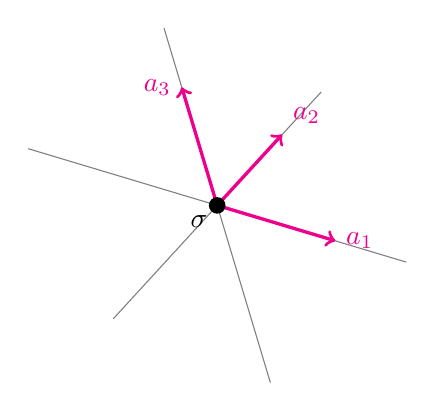
\begin{tikzpicture}[x = {(1cm, 0cm)}, y = {(0.55cm, 0.4cm)}, z = {(0cm, 1cm)}, scale = 1.5]
            \draw[gray] (-1.6, 0, 0.48) -- (1.6, 0, -0.48);
            \draw[gray] (0, -1.6, -0.32) -- (0, 1.6, 0.32);
            \draw[gray] (0.45, 0, -1.5) -- (-0.45, 0, 1.5);
            \draw[very thick, magenta, ->] (0, 0, 0) -- (1, 0, -0.3) node[right] {$a_1$};
            \draw[very thick, magenta, ->] (0, 0, 0) -- (0, 1, 0.2) node[above right] {$a_2$};
            \draw[very thick, magenta, ->] (0, 0, 0) -- (-0.3, 0, 1) node[left] {$a_3$};
            \fill[black] (0, 0, 0) circle (2pt) node[below left] {$\sigma$};
        \end{tikzpicture}
    \end{figure}

    % [FILLED] the reason the directional derivatives vanish was a \todo{why?}
    The directional derivatives of $p$ at $\sigma$ in all these directions $a_1, a_2, a_3$ must be zero. Indeed, $p$ vanishes on the line $\setst{a_i t + \sigma}{t \in \R}$, so $t \mapsto p\of{a_i t + \sigma}$ is the zero polynomial, and its derivative at $t = 0$, which by the chain rule is $\cycl{\nabla p (\sigma), a_i}$, is zero. So $\nabla p (\sigma)$ must itself be zero, because its inner product with all elements of a basis is zero. In particular, all three partial derivatives also vanish at every joint. But this necessitates that either one of these is a nonzero polynomial of smaller degree than $p$ or $p$ is the zero polynomial. Either way, we have a contradiction.
\end{proof}

Using the lemma, we notice that
\begin{align*}
    J(L)
    &\leq J(L - 1) + 3J(L)^{\frac{1}{3}} \\
    &\leq J(L - 2) + 3 \cdot 2 \cdot J(L)^{\frac{1}{3}} \\
    &\leq J(L - 3) \cdots \\
    &\leq 3 \cdot L \cdot J(L)^{\frac{1}{3}}
\end{align*}
The first inequality comes from taking $L$ lines with $J(L)$ joints and deleting a line that, by the lemma, is in at most $3J(L)^{\frac{1}{3}}$ of them; every other joint survives. Repeating this, and using $J(L - 1) \leq J(L)$, each of the $L$ deletions costs at most $3J(L)^{\frac{1}{3}}$ joints, which is the last line. Rearranging gives $J(L) \leq \parenth{3L}^{\frac{3}{2}}$.
